% !TEX root = paper/paper.tex
\vspace{-1em}
\begin{abstract}
Humans are capable of perceiving a scene at a glance, and obtain deeper understanding with additional time. Similarly, visual recognition deployments should be robust to varying computational budgets. Such situations require Anytime recognition ability, which is rarely considered in computer vision research. We present a method for learning dynamic policies to optimize Anytime performance in visual architectures. Our model sequentially orders feature computation and performs subsequent classification. Crucially, decisions are made at test time and depend on observed data and intermediate results. We show the applicability of this system to standard problems in scene and object recognition. On suitable datasets, we can incorporate a semantic back-off strategy that gives maximally specific predictions for a desired level of accuracy; this provides a new view on the time course of human visual perception.
\end{abstract}

%
\section{Introduction} \label{sec:intro}
%
%
\looseness -1 In many  problems arising in artificial intelligence one
needs to adaptively make a sequence of decisions, taking into account
observations about the outcomes of past decisions.  Often these
outcomes are uncertain, and one may only know a probability
distribution over them.  Finding optimal policies for decision making
in such partially observable stochastic optimization problems is
notoriously intractable (see, e.g., \citet{littman98computational}).  A fundamental challenge is to identify classes of planning problems for which simple solutions obtain (near-) optimal performance.


In this paper, we 
introduce the concept of \emph{\term submodularity}, and prove that
if a partially observable stochastic optimization problem satisfies this property, a simple adaptive greedy
algorithm is guaranteed to obtain near-optimal solutions. In fact, under reasonable complexity-theoretic assumptions, no polynomial time algorithm is able to obtain better solutions in general.
\Term
  submodularity generalizes the classical notion of submodularity\footnote{For
  an extensive treatment of submodularity, see the books
  of~\citet{fujishige05} and~\citet{SchrijverB}.}, which has
been successfully used to develop approximation algorithms for a
variety of non-adaptive optimization problems. 
 Submodularity, informally, is an intuitive notion of diminishing
 returns, which states that adding an element to a small set helps
 more than adding that same element to a larger (super-)\ set.  A
 celebrated result of the work of~\citet{nemhauser78} guarantees that for such
 submodular functions, a simple greedy algorithm, which adds the element that maximally increases the objective value, selects a near-optimal set of $k$ elements.  
Similarly, it is guaranteed to find a set of near-minimal cost that
achieves a desired quota of utility~\citep{wolsey82}, using 
near-minimum average time to do so~\citep{streeter08}.
Besides guaranteeing theoretical performance bounds, submodularity allows us
to speed up algorithms without loss of solution quality by using lazy evaluations \citep{minoux78},
often leading to performance improvements of several orders of
magnitude \citep{leskovec07}.  Submodularity has been shown to be very useful in a variety of problems in artificial intelligence \citep{krause09ijcaitut}.

The challenge in generalizing
submodularity to adaptive planning --- where the action taken in each
step depends on information obtained in the previous steps  --- is that feasible solutions are now
policies (decision trees or conditional plans) instead of subsets. We propose a natural
generalization of the diminishing returns property for adaptive
problems, which reduces to the classical characterization of submodular set
functions for deterministic distributions. We show how these results
of~\citet{nemhauser78},~\citet{wolsey82},~\citet{streeter08},
and~\citet{minoux78} generalize to the adaptive setting.  Hence,
we demonstrate how \term submodular optimization problems enjoy
theoretical and practical benefits similar to those of classical,
nonadaptive submodular problems. We further demonstrate the usefulness
and generality of the concept by showing how it captures known results
in stochastic optimization and active learning as special cases,
admits tighter performance bounds,  leads to natural generalizations
and allows us to solve new problems for which no performance guarantees were known.

As a first example, consider the problem of deploying (or controlling) a collection of
sensors to monitor some spatial phenomenon. Each sensor can cover a
region depending on its sensing range. Suppose we would like to find
the best subset of $k$ locations to place the sensors.  In this
application, intuitively, adding a sensor helps more if we have placed
few sensors so far and helps less if we have already placed many sensors. We can formalize this diminishing returns property using the notion of submodularity --
the total area covered by the sensors is a submodular function defined
over all sets of locations.  \citet{krause07nearoptimal} show that
many more realistic utility functions in sensor placement (such as the
improvement in prediction accuracy w.r.t.~some probabilistic model)
are submodular as well. Now consider the following stochastic variant:
Instead of deploying a fixed set of sensors, we deploy one sensor at a
time.  With a certain probability, deployed sensors can fail, and our
goal is to maximize the area covered by the functioning sensors.
Thus, when deploying the next sensor, we need to take into account
which of the sensors we deployed in the past failed.  This problem has
been studied by \citet{AsadpourNS08} for the case where each sensor
fails independently at random.  In this paper, we show that the
coverage objective is \term submodular, and use this concept to handle
much more general settings (where, e.g., rather than all-or-nothing
failures there are different types of sensor failures of varying severity).
%
We also consider a related problem where the goal is to place the minimum number of
sensors to achieve the maximum possible sensor coverage (i.e., the coverage
obtained by deploying sensors everywhere), or more generally the
goal may be to achieve any fixed percentage of the maximum possible
sensor coverage.  
Under the first goal, the problem is equivalent to one studied by~\citet{goemans06stochastic}, and 
generalizes a problem studied by \citet{liu08near}.  As with the
maximum coverage version, \term submodularity 
allows us to recover and generalize previous results.
 


As another example, consider a viral marketing problem, where we are
given a social network, and we want to influence as many people as
possible in the network to buy some product. We do that by giving the
product for free to a subset of the people, and hope that they
convince their friends to buy the product as well.  Formally, we have
a graph, and each edge $e$ is labeled by a number $0\leq p_e\leq 1$.  We ``influence'' a subset of nodes in the graph, and for each influenced node, their neighbors get randomly influenced according to the probability annotated on the edge connecting the nodes.  This process repeats until no further node gets influenced.  \citet{kempe03} show that the set function which quantifies the expected number of nodes influenced is submodular.  A natural stochastic variant of the problem is where we pick a node, get to see which nodes it influenced, then adaptively pick the next node based on these observations and so on.  We show that a large class of such adaptive influence maximization problems satisfies \term submodularity.


Our third application is in active learning, 
where we are given an unlabeled data set, and we would like to
adaptively pick a small set of examples whose labels imply all other
labels.  The same problem arises in automated diagnosis, where we have
hypotheses about the state of the system (e.g., what illness a patient has), and would like to perform tests to identify the correct hypothesis.
In both domains we want to pick examples / tests to shrink the remaining
version space (the set of consistent hypotheses) as quickly as
possible. Here, we show that the reduction in version space
probability mass is
\term submodular, and use that observation to prove that the adaptive
greedy algorithm is a near-optimal querying policy, recovering and 
%
generalizing  
results by \citet{kosaraju99} and~\citet{dasgupta04}. Our results for active learning and automated diagnosis are also related to recent results of \citet{guillory10interactive,guillory2011-noisy-interactive-submod-cover} who study generalizations of submodular set cover to an interactive setting.  In contrast to our approach however, \citeauthor{guillory10interactive} analyze worst-case costs, and use rather different technical definitions and proof techniques.


We summarize our main contributions below, and provide a more
technical summary in  Table~\ref{table:results}.
At a high level, our main contributions are: 
\begin{itemize}
\item We consider a particular class of partially observable adaptive stochastic optimization problems, which we prove to be hard to approximate in general.
\item We introduce the concept of \emph{\term submodularity}, and
  prove that if a problem instance satisfies this property, a simple
  adaptive greedy policy performs near-optimally, for both adaptive
  stochastic maximization and coverage, and also a natural min-sum objective.
\item We show how \term submodularity can be exploited by allowing the
  use of an accelerated adaptive greedy algorithm using lazy
  evaluations, and how we can obtain data-dependent bounds on the optimum.
\item We illustrate \term submodularity on several realistic problems,
  including Stochastic Maximum Coverage, Stochastic Submodular Coverage,
  Adaptive Viral Marketing, and 
  Active Learning.  For these applications, \term submodularity allows
  us to recover known results and prove natural generalizations.
\end{itemize}

%
%
\newcommand{\AS}{A.S.\xspace}
\newcommand{\AMS}{A.M.S.\xspace}

\begin{table}[t]
%
  \begin{tabular}{|p{1.5in}|p{3.4in}|p{0.8in}|}
\hline
\hspace{0.5in} {\bf Name} & \hspace{1.15in} {\bf New Results} &
\hspace{3mm} {\bf Location} \\ %
\hline
\AS Maximization & Tight $(1-1/e)$-approx.\ for \AMS objectives &
\secref{ssec:max-cover-objective}, page~\pageref{ssec:max-cover-objective}\\
\hline
\AS Min Cost Coverage & Tight logarithmic approx.\ for \AMS
objectives & \secref{sec:min-cost-cover}, page~\pageref{sec:min-cost-cover}\\
\hline
\AS Min Sum Cover & Tight $4$-approx.\ for \AMS objectives &
\secref{sec:min-sum-cover}, page~\pageref{sec:min-sum-cover}\\
\hline
Data Dependent Bounds & Generalization to
\AMS functions & \secref{ssec:max-cover-objective}, page~\pageref{ssec:max-cover-objective}\\
\hline
Accelerated Greedy & Generalization of lazy evaluations to the
adaptive setting & \secref{sec:the-greedy-policy}, page~\pageref{sec:the-greedy-policy}\\
\hline    
Stochastic Submodular Maximization &  Generalization of the previous $(1-1/e)$-approx.\ to \mbox{arbitrary} 
per--item set distributions, and to item costs &
\secref{sec:stochastic-maximization}, page~\pageref{sec:stochastic-maximization}\\
\hline    
Stochastic Set Cover & Generalization of the previous
$(\ln(n)+1)$-approx.\ to \mbox{arbitrary} per-item set distributions, with
item costs & \secref{sec:stochastic-set-cover}, page~\pageref{sec:stochastic-set-cover}\\
\hline    
\mbox{Adaptive Viral} \mbox{Marketing} & Adaptive analog of previous
$(1-1/e)$-approx.\ for non-adaptive viral marketing, under more
general reward functions; tight logarithmic approx.\ for the adaptive
min cost cover version & \secref{sec:viral-marketing}, page~\pageref{sec:viral-marketing}\\
\hline    
Active Learning & Improved approx.\ factor of generalized binary search and its approximate versions
%
with and without item costs & \secref{sec:active-learning}, page~\pageref{sec:active-learning}\\
\hline    
%
%
Hardness in the absence of Adapt.\ Submodularity &
$\Omega(|\groundset|^{1-\epsilon})$-approximation hardness for \AS
Maximization, Min Cost Coverage, and Min-Sum Cover, if $f$ is not
\term submodular.  & \secref{sec:hardness}, page~\pageref{sec:hardness}\\
\hline    
 \end{tabular}
  \caption{Summary of our theoretical results.  \AS is shorthand for
    ``adaptive stochastic'', and \AMS is shorthand for ``adaptive
    monotone submodular.'' \vspace{-5mm}}  \label{table:results}
\end{table}


%
%
%
%


\subsection{Organization} %

\looseness -1 This article is organized as follows.
In \secref{sec:problem-statment} (page~\pageref{sec:problem-statment}) we set up notation and formally define
the relevant adaptive optimization problems for general objective
functions. 
\emph{For the reader's convenience, we have also provided a reference table of
important symbols on page~\pageref{table:symbol-table}.}
In~\secref{sec:term-submodularity} (page~\pageref{sec:term-submodularity}) we review the classical notion of submodularity and introduce the novel 
\term submodularity property.  In~\secref{sec:the-greedy-policy}
(page~\pageref{sec:the-greedy-policy}) we introduce
the adaptive greedy policy, as well as an accelerated variant.
In~\secref{sec:greedy} (page~\pageref{sec:greedy}) we discuss the theoretical guarantees
that the adaptive greedy policy enjoys when applied to 
problems with \term submodular objectives.
Sections~\ref{sec:stochastic-maximization} through~\ref{sec:active-learning}
provide examples on how to apply the \term submodular framework to
various applications, namely Stochastic Submodular Maximization
(\secref{sec:stochastic-maximization}, page~\pageref{sec:stochastic-maximization}), Stochastic Submodular Coverage
(\secref{sec:stochastic-set-cover}, page~\pageref{sec:stochastic-set-cover}), 
Adaptive Viral Marketing (\secref{sec:viral-marketing}, page~\pageref{sec:viral-marketing}), and 
Active Learning (\secref{sec:active-learning}, page~\pageref{sec:active-learning}).
In~\secref{sec:experiments} (page~\pageref{sec:experiments}) we report empirical results on two sensor
selection problems.
In~\secref{sec:adaptgap} (page~\pageref{sec:adaptgap}) we discuss the adaptivity gap of the problems we
consider, and in~\secref{sec:hardness} (page~\pageref{sec:hardness}) we prove hardness results
indicating that problems which are not \term submodular  can be extremely
inapproximable under reasonable complexity assumptions.
We review related work in~\secref{sec:related-work} (page~\pageref{sec:related-work}) and provide concluding remarks in
\secref{sec:conclusions} (page~\pageref{sec:conclusions}).  \AppendixA (page~\pageref{sec:proofs}) gives details of how to incorporate item
costs and includes all of the proofs omitted from the main text. 



%
%
%
%
%

% !TEX root = paper/paper.tex
\section{Related Work}
% \paragraph{Feature combination and selection.}
% \emph{Boosting} is a method for combining weak learners into a more powerful classifier \cite{Hastie2009}.
% A popular use of boosting is in introducing non-linearities by training depth-limited decision trees as weak learners---the boosting trick.
% For SVM-based classifiers, \emph{Multiple Kernel Learning} (MKL) provides a way to train classifiers using an automatically weighted combination of kernels \cite{Lanckriet2004}.
% It has been shown that MKL is outperformed by boosting single-kernel classifiers \cite{Gehler2009}.
% Of course, if all classifiers are linear, then combining outputs of classifiers trained on different feature channel with another classifier is equivalent to training one classifier on all features at once.
% \todo{What about learning a \emph{non-linear} second classifier on top of the weak learner scores---any papers?}

% \todo{A couple of sentences on feature selection approaches, particularly using infogain as proxy for classification error.}

\paragraph{Static selection}% test-time efficient feature selection.}
% The simplest way to limit the number of features used at test time is to $L_1$-regularize.
% This method does not explicitly consider feature cost, nor is it able to evaluate features one by one, or to give an answer before all features are computed.

A well-known method to evaluate features sequentially is the cascaded boosted classifier of Viola \& Jones \cite{Viola2004} (updated by Bourdev \& Brandt \cite{Bourdev-CVPR-2005} with a soft threshold), which is able to quit evaluating an instance before all features are computed---but feature cost was not considered.
The cost-sensitive cascade of Chen et al.\ \cite{Chen-AISTATS-2012} optimizes stage order and thresholds to jointly minimize classification error and feature computation cost.
Xu et al.\ \cite{Xu-ICML-2012} and Grubb \& Bagnell \cite{Grubb-AISTATS-2012} separately develop a variant of gradient boosting for training cost-sensitive classifiers; the latter prove near-optimality of their greedy algorithm with submodularity results.
Their methods are tightly coupled to the stage-wise regression algorithm.

\vspace{-1em}
\paragraph{Dynamic selection}% test-time efficient feature selection.}
The above methods learn an efficient but \emph{fixed} order for evaluating features given a test instance.

Gao \& Koller \cite{Gao-NIPS-2011} propose a method for \emph{active classification}: myopically selecting the next feature based on expected information gain given the values of the already selected features.
The method is based on locally weighted regression, highly costly at test time.
Ji \& Carin \cite{Ji-PR-2007} also formulate cost-sensitive feature selection generatively, as an HMM conditioned on actions, but select actions myopically, again at signficant test time cost.

Karayev at al.\ \cite{Karayev-NIPS-2012} propose a reinforcement learning approach for selecting object detectors; they rely on expensive test-time inference in a graphical model to combine observations.
Dulac-Arnold et al.\ \cite{Dulac-Arnold-ML-2012} present another MDP-based solution to ``datum-wise classification'', with an action space comprised of all features and labels, recently extended to region-based processing \cite{Dulac-Arnold-ICLR-2014}.
He He et al.\ \cite{HeHe-ICMLW-2012} also formulate an MDP with features and a single classification step as actions, but solve it via imitation learning of a greedy policy.
Benbouzid et al.\ \cite{Benbouzid-ICML-2012} formulate an MDP that simply extends the traditional sequential boosted classifier with an additional \emph{skip} action, significantly limiting the space of learnable policies (\cite{Trapeznikov} provides another variation on this problem).
Although \cite{Karayev-NIPS-2012} targets \emph{Anytime} performance, their inference procedure is prohibitively expensive for test-time use in a general classification task.
In contrast, our fast linear method allows direct specification of the Anytime cost budget.

\emph{Label trees} also guide an instance through a tree of classifiers; their structure is determined by the confusion matrix or learned jointly with weights \cite{Deng-NIPS-2011}.
Xu et al.\ \cite{Xu-ICML-2013} learn a cost-sensitive binary tree of weak learners using an approach similar to the cyclic optimization of \cite{Chen-AISTATS-2012}.
Less directly related---but exciting for its novelty---is the work of \cite{weiss2013dynamic}, who apply simple introspection to structured models for a significant speedup of human pose estimation.
Another exciting direction is theoretical analysis of near-optimal policies with humans in the loop \cite{chen14active}.

% !TEX root = paper/paper.tex

\begin{figure}[t]
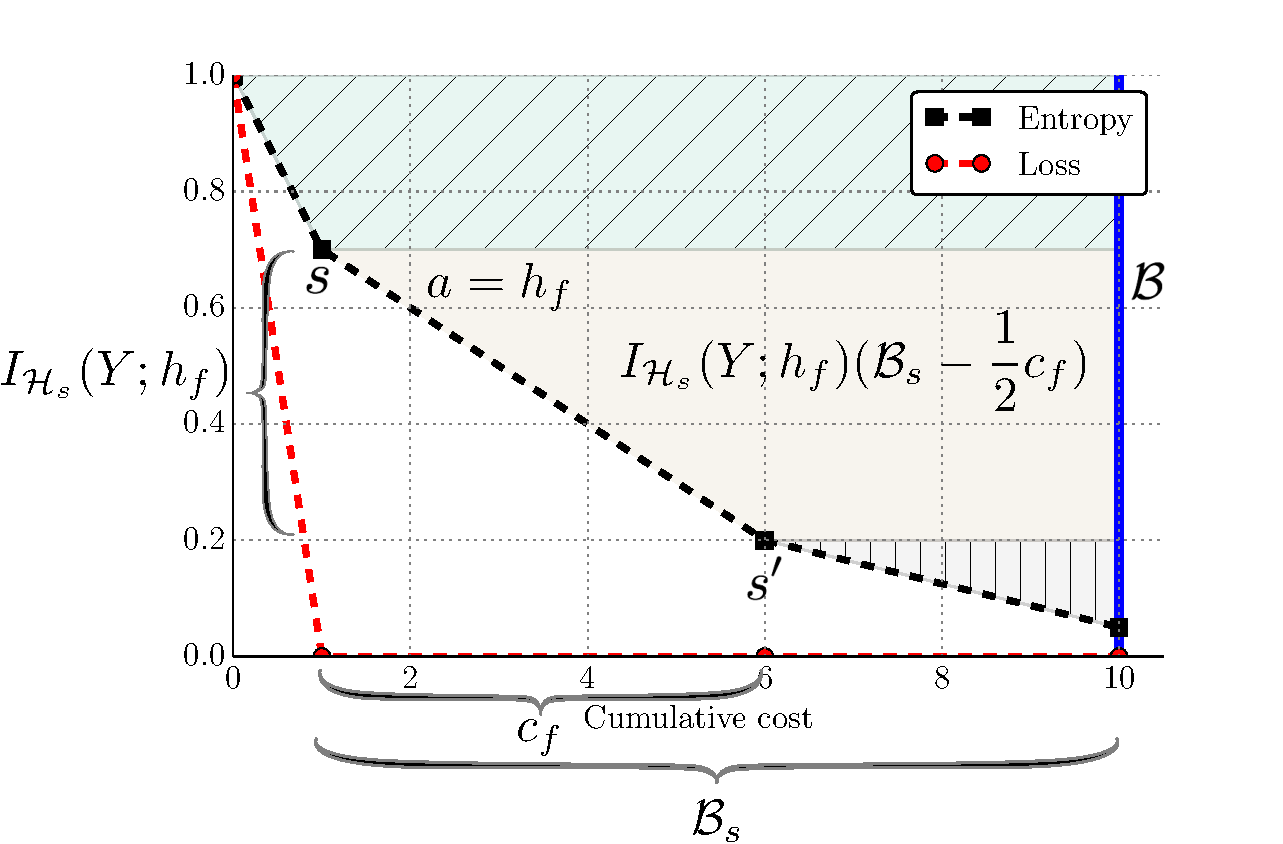
\includegraphics[width=1\linewidth]{../../figures/rewards.pdf}
\caption{
Definition of the reward function.
To maximize the total area above the entropy vs. cost curve from $0$ to $\mathcal{B}$, we define the reward of an individual action as the area of the slice of the total area that it contributes.
From state $s$, action $a = h_f$ leads to state $s'$ with cost $c_f$.
The information gain is $I_{\mathcal{H}_s}(Y; h_f) = H(Y; \mathcal{H}_s) - H(Y; \mathcal{H}_s \cup {h_f})$.
\label{fig:rewards}}
\end{figure}

\section{Anytime Classification by Cost-sensitive\\Dynamic Feature Selection}

\begin{mydef} \label{def:problem}
\textbf{The test-time efficient multi-class classification problem} consists of

\begin{itemize}
\addtolength{\itemsep}{-.55\baselineskip}
\item
$N$ instances labeled with one of $K$ labels: ${\mathcal{D} = \{x_n \in \mathcal{X}, y_n \in \mathcal{Y} = \{1, \dots, K\}\}_{n=1}^N}$.

\item
$F$ features $\mathcal{H} = \{h_f : \mathcal{X} \mapsto \mathbb{R}^{d_f} \}_{f=1}^F$, with associated costs $c_f$.

\item Budget-sensitive loss $\mathcal{L}_\mathcal{B}$, composed of cost budget $\mathcal{B}$ and loss function ${\ell(\hat{y}, y) \mapsto \mathbb{R}}$.
\end{itemize}

The goal is to find a \textbf{feature selection} policy $\pi(x): \mathcal{X} \mapsto 2^\mathcal{H}$ and a \textbf{feature combination} classifier $g(\mathcal{H}_\pi) : 2^\mathcal{H} \mapsto \mathcal{Y}$ such that such that the total budget-sensitive loss $\sum \mathcal{L}_\mathcal{B}(g(\pi(x_n)), y_n)$ is minimized.
\end{mydef}

%The features $h_f$ can be classifier outputs, possibly multi-class; following convention, we refer to such features as \emph{weak learners}.

The cost of a selected feature subset $\mathcal{H}_{\pi(x)}$ is $C_{\mathcal{H}_\pi(x)}$.
The budget-sensitive loss $\mathcal{L}_\mathcal{B}$ presents a \textbf{hard budget constraint} by only accepting answers with $C_{\mathcal{H}} \leq \mathcal{B}$.
Additionally, $\mathcal{L}_\mathcal{B}$ can be \textbf{cost-sensitive}: answers given with less cost are more valuable than costlier answers.
The motivation for the latter property is \emph{Anytime} performance; we should be able to stop our algorithm's execution at any time and have the best possible answer.

Feature costs $c_f$ can be specified flexibly, with options including theoretical analysis, number of flops, wall clock runtime, total CPU time, or exact power expenditure.
We believe that a deployment in a modern datacenter is most likely to optimize for power expenditure.
In the absence of reliable ways to measure power, we use total CPU time to define the cost: if an operation is performed in parallel on multiple cores, its cost is considered to be the total cpu time on all cores.

% For a weak learner $h_f$, the cost $c_f$ is composed of the cost of an underlying feature extraction $\phi_{h_f}(x)$ and the cost of subsequent classification.
% Once $h_f$ is computed, its underlying feature $\phi$ is considered to be free for all other features $h_f'$ that share it, if any, such that $c_f' < c_f$.
% Note that in state-of-the-art object recognition systems, complex features and feature encodings are often followed by linear classifiers, and feature extraction cost dominates the total cost.

% \todo{REDO this:}
% A quick preview of an instance of the defined problem is in order.
% On the ImageNet dataset, we could define $h_f$ as intersections of feature channels and class subsets:\\
% {\footnotesize\texttt{
% GIST.Animal, SIFT-BOW.Animal, LLC-SIFT.Animal,\\
% GIST.Vehicle, SIFT-BOW.Vehicle, LLC-SIFT.Vehicle.}}\\
% $\mathcal{G}$ could be defined by a hierarchical loss (accuracy at the leaf nodes counts more than accuracy at inner nodes), and $\mathcal{B}$ could only admit answers that take less than 5 seconds.

At training time, our computation is unbudgeted, and we can compute all features to have \emph{fully-observed} training instances.
At test time, there is a budget and so the instances we classify will only be \emph{partially-observed}, as determined by the feature selection policy.

We defer discussion of learning the \textbf{feature combination} classifier $g(\mathcal{H}_\pi) : 2^\mathcal{H} \mapsto \mathcal{Y}$ to~\autoref{sec:classifier}.
For now, we assume that $g$ can combine an arbitrary subset of features and provide a distribution $P(Y = y)$.
For example, $g$ could be a Naive Bayes (NB) model trained on the fully-observed data.

% \subsection{Static greedy selection.}
% Our initial goal is select a feature subset $\pi(x)$ such that $C_{\pi(x)} \leq \mathcal{B}$ and $\sum \ell(g(\pi(x_n)), y_n)$ is minimized.
% We assume that given a feature subset $\pi(x)$, we are able to find a classifier function $g$ such that the loss is minimized.

% If the classifier $g$ can give a full distribution $P(Y = y)$ and not just a prediction $y \in \{1, \dots, K\}$, we can maximize information gain of the selected subset, instead of directly minimizing the loss of $g(\pi(x))$:\[
% I(Y; \pi(x)) = H(Y) - H(Y | \pi(x)) = \sum_{y \in Y} P(y) \log P(y) -  \sum_{\substack{y \in Y,\\z \in Z}} P(y, z) \log P(y \mid z)
% \]
% To the extent that $g$ is unbiased, maximizing information gain corresponds to minimizing loss, and has the benefit of ensuring that we not only make the right classification decision but also become maximally certain.

% Finding the optimal subset is NP-hard.
% A common heuristic is simple greedy selection, which is known to be near-optimal for optimizing submodular set functions with unit-cost elements \cite{Nemhauser-1978}.
% In case of non-uniform additive costs, it can be proven that when all features $h$ are independent given $Y$ (as in an NB classifier), building $\pi(x)$ by repeatedly selecting
% \begin{align*}
% h* = \argmax_{h \in \mathcal{H} \setminus \pi(x)} \frac{1}{c_f} \left[ H(h \mid \pi(x)) - H(h \mid Y) \right]
% \end{align*}
% while $C_{\pi(x)} \leq \mathcal{B}$ gives $I(Y; \pi(x)) \geq \frac{1}{2} (1 - 1/e) I_{\text{OPT}}$ with additional terms if the entropy calculation is not exact \cite{Krause-UAI-2005}\footnote{A tighter (by factor of 2) bound is possible with a $O(F^5)$ instead of this $O(F^2)$ algorithm \cite{Krause-note-2005}.}.

% However, we may find the feature independence assumption too restrictive or may not be able to reliably compute entropy.
% Additional difficulties come from introducing a setup cost or non-additive costs \todo{although we could resolve them.}
% When we make the feature selection dynamic---guided by the feature values observed---we will face further challenges if the structure of the problem necessitates a non-myopic solution.
% \todo{Need stronger explanation for why we are not proceeding with adaptive submodularity---or just not mention submodularity at all?}

\subsection{Dynamic feature selection as a Markov-Decision-Process (MDP).}
To model the \textbf{feature selection} policy $\pi(x): \mathcal{X} \mapsto 2^\mathcal{H}$, we introduce the Markov Decision Process (MDP), which defines a single \emph{episode} of selecting features for some instance $x$.

\begin{mydef} \label{def:MDP}
The \textbf{feature selection MDP} consists of the tuple $(\mathcal{S}, \mathcal{A}, T(\cdot), R(\cdot), \gamma)$:

\begin{itemize}\addtolength{\itemsep}{-.55\baselineskip}
\item \textbf{State} $s \in \mathcal{S}$ stores the selected feature subset $\mathcal{H}_{\pi(x)}$ and their values and total cost $C_{\mathcal{H}_{\pi(x)}}$.
\item The set of \textbf{actions} $\mathcal{A}$ is exactly the set of features $\mathcal{H}$.
\item The (stochastic) \textbf{state transition} distribution $T(s' \mid s, a)$ can depend on the instance $x$.
\item The \textbf{reward} function $R(s, a, s') \mapsto \mathbb{R}$ is manually specified, and depends on the classifier $g$ and the instance $x$.
\item The discount $\gamma$ determines amount of \textbf{lookahead} in selecting actions: if 0, actions are selected greedily based on their immediate reward; if 1, the reward accrued by subsequent actions is given just as much weight as the reward of the current action.
\end{itemize}
\end{mydef}

Running the MDP on a given instance $x$ gives a trajectory $\xi = (s_0, a_0, s_1, r_1, \dots, a_{I-1}, s_I, r_I)$, where $I$ is the total number of actions taken (and therefore features selected), $s_0$ is the initial state, $a_i \sim \pi(a \mid s_i)$ is chosen by the \emph{policy} $\pi(a \mid s)$, and $s_{i+1} \sim T(s \mid s_i, a_i)$, which can depend on $x$.
The total expected reward (value) of an MDP episode is written as
\begin{equation} \label{eq:expected_reward}
V_\pi(s_0) =
\mathbb{E}_{\xi \sim \left\{ \pi, x \right\}} r(\xi) =
\mathbb{E}_{\xi \sim \left\{ \pi, x \right\}} \left[ \sum_{i=0}^I \gamma^i \, r_i \right]
\end{equation}
Gathering such trajectories forms the basis of our policy learning method.

\subsection{Defining the reward.}
The budget-sensitive loss $\mathcal{L}_\mathcal{B}$ enforces \emph{Anytime} performance by valuing early gains more than later gains.
To formalize this, consider \hyperref[fig:rewards]{Figure~\ref*{fig:rewards}}, which shows the entropy and the 0-1 loss of $g$ at every point in a sequential feature selection episode for some instance $x$.
For the best \emph{Anytime} performance, we want to capture the most area above the loss vs. cost curve, up to max budget $\mathcal{B}$ \cite{Karayev-NIPS-2012}.

Recall from \eqref{eq:expected_reward} that the value of an episode $\xi$ is defined as the sum of obtained rewards.
If the reward of a single action is defined as the area above the curve that is captured as a direct result, then the value of the whole episode exactly corresponds to $\mathcal{L}_\mathcal{B}$.

However, there is a problem with using loss directly: only the first action to ``tip the scale'' toward the correct prediction gets a direct reward (in the figure, it is the first action).  A smoother reward function is desirable:
if the classifier $g$ can give a full distribution $P(Y = y \mid \mathcal{H}_{\pi(x)})$ and not just a prediction $\hat{y} \in \mathcal{Y}$, we can maximize the \emph{information gain} of the selected subset instead of directly minimizing the loss of $g(\pi(x))$:
\begin{eqnarray}
I(Y; \mathcal{H}_{\pi(x)}) &=& H(Y) - H(Y | \mathcal{H}_{\pi(x)}) = \\ \notag
&=& \sum_{y \in Y} P(y) \log P(y) -  \\ \notag
&&\sum_{y, \mathcal{H}_{\pi(x)}} P(y, \mathcal{H}_{\pi(x)}) \log P(y \mid \mathcal{H}_{\pi(x)})
\end{eqnarray}
To the extent that $g$ is unbiased, maximizing information gain corresponds to minimizing loss, and ensures that we not only make the right classification decision but also become maximally certain.
Therefore, as graphically presented in \hyperref[fig:rewards]{Figure~\ref*{fig:rewards}}, we define the reward of selecting feature $h_s$ with cost $c_f$ with the set $\mathcal{H}_s$ computed to be $I_{\mathcal{H}_s}(Y; h_f) (\mathcal{B}_s - \frac{1}{2}c_f)$.

Although we do not evaluate in this regime, note that this definition easily incorporates a \textbf{setup cost} in addition to \textbf{deadline cost} by only computing the area in between setup and deadline costs.

\subsection{Parametrizing and learning the policy.}
% From the trajectories we can compute the \emph{value function} for any state:
% \begin{equation} \label{eq:value_function}
% V_\pi(s) = \sum_{s'} T_\pi(s, s') \left[ R_\pi(s, s') + \gamma V_\pi(s') \right]
% \end{equation}

Space constraints prohibit a full exposition of reinforcement learning techniques; \cite{Sutton1998} provides a thorough review.
In brief: we seek $\pi$ that maximizes the expected value of the MDP \eqref{eq:expected_reward}.
Therefore, actions must be selected according to their expected \emph{value}:
\begin{align*}
\argmax_a \pi(a \mid s) = \argmax_a Q^*(s,a)
\end{align*}
where $Q^*(s,a)$ is the optimal \emph{action-value function}---the expected value of taking action $a$ in state $s$ and then acting optimally to the end of the episode.

Because the state represents an exponential number of subsets and associated real values, we cannot represent $Q(s,a)$ exactly.
Instead, we use feature approximation and write $Q(s,a) = \theta^T \phi(s, a)$,  where $\phi: \mathcal{S} \times \mathcal{A} \mapsto \mathbb{R}^{d_s}$ is the state featurization function, $d_s$ is the dimensionality of the state feature vector, and $\theta$ is a vector of weights that defines the policy.

Specifically, the policy is defined as
\begin{equation}
\pi(a \mid s) = \frac{1}{Z} \exp\left(\frac{1}{\tau} \theta^T \phi(s, a)\right)
\end{equation}
where $Z$ is the appropriate normalization and $\tau$ is a temperature parameter that controls the level of exploration vs. exploitation in the policy.
As $\tau \rightarrow 0$, ${\pi(a \mid s)}$ becomes highly peaked at $\argmax_a Q(s,a)$; it becomes uniform as $\tau \rightarrow \infty$.

As commonly done, we learn the $\theta$ by \emph{policy iteration}.
First, we gather $(s, a, r, s')$ samples by running episodes (to completion) with the current policy parameters $\theta_i$.
From these samples, $\hat{Q}(s, a)$ values are computed, and $\theta_{i+1}$ are given by $L_2$-regularized least squares solution to $\hat{Q}(s, a) = \theta^T \phi(s, a)$, on all states that we have seen in training.

During training, we gather samples starting from either a random feasible state, with probability $\epsilon$, or from the initial empty state otherwise.
Both $\epsilon$ and $\tau$ parameters decay exponentially with the number of training iterations.
Training is terminated if $\pi_{\theta_{i+1}}$ returns the exact same sequence of episodes $\xi$ on a validation set as $\pi_{\theta_{i}}$.

\vspace{-1em}
\paragraph{Static vs. Dynamic state-action feature vector.}\label{sec:policy_features}
The featurization function $\phi(s)$ extracts the following features from the state:
\begin{itemize}\addtolength{\itemsep}{-.5\baselineskip}
\item Bit vector $\textbf{m}$ of length $F$: initially all bits are $1$ and are set to $0$ when the corresponding feature is computed.
\item For each $h_f$, a vector of size $d_f$ representing the values; $0$ until observed.
\item Cost feature $c \in [0, 1]$, for fraction of the budget spent.
\item Bias feature $1$.
\end{itemize}

\begin{algorithm}[]
\SetKwFunction{ComputeRewards}{ComputeRewards}
\SetKwFunction{GatherSamples}{GatherSamples}
\SetKwFunction{UpdatePolicy}{UpdatePolicy}
\SetKwFunction{UpdateClassifier}{UpdateClassifier}

\SetAlgoLined
\KwIn{$\mathcal{D} = \{x_n, y_n\}_{n=1}^N$; $\mathcal{L}_\mathcal{B}$}
\KwResult{Trained $\pi$, $g$}
\BlankLine
$\pi_0 \leftarrow$ random\;
\For {$i \leftarrow 1$ \KwTo max\_iterations} {
    States, Actions, Costs, Labels $\leftarrow$ \GatherSamples{$\mathcal{D}$, $\pi_{i-1}$}\;
    $g_i \leftarrow$ \UpdateClassifier{States, Labels}\;
    Rewards $\leftarrow$ \ComputeRewards{States, Costs, Labels, $g_i, \mathcal{L}_\mathcal{B}, \gamma$}\;
    $\pi_i \leftarrow$ \UpdatePolicy{States, Actions, Rewards}\;
}
\caption{Because reward computation depends on the classifier, and the distribution of states depends on the policy, $g$ and $\pi$ are trained iteratively.\label{alg:learning}}
\end{algorithm}

These features define the \textbf{dynamic} state, presenting enough information to have a \emph{closed-loop} (dynamic) policy that may select different features for different test instances.
The \textbf{static} state has all of the above features except for the observed feature values.
This enables only an \emph{open-loop} (static) policy, which is exactly the same for all instances.
Policy learned with the static state is used as a baseline in experiments.

The state-action feature function $\phi(s, a)$ effectively block-codes these features: it is $0$ everywhere except the block corresponding to the action considered.
In implementation, we train $F$ separate regressions with a tied regularization parameter, which is K-fold cross-validated.

\paragraph{Effect of $\gamma$.}
Note that solving the MDP with these features and with $\gamma=0$ finds a \textbf{Static, greedy} policy: the value of taking an action in a state is exactly the expected reward to be obtained.
When $\gamma=1$, the value of taking an action is the entire area above the curve as defined in \autoref{fig:rewards}, and we learn the \textbf{Static, non-myopic} policy---another baseline.

\subsection{Learning the classifier.}\label{sec:classifier}

We have so far assumed that $g$ can combine an arbitrary subset of features and provide a distribution $P(Y = y)$---for example, a Gaussian Naive Bayes (NB) model trained on the fully-observed data.
% However, a Naive Bayes classifier suffers from its restrictive independence assumptions.

Since discriminative classifiers commonly provide better performance, we use a \textbf{logistic regression} classifier, which presents a new challenge:
% bu have to account for missing data:
at test time, some feature values are missing and need to be imputed.
If the classifier is trained exclusively on fully-observed data, then the feature value statistics at test time will not match, resulting in poor performance.
Therefore, we need to learn classifier weights on a distribution of data that exhibits the pattern of missing features induces by the policy $\pi$.
At the same time, learning the policy depends on the classifier $g$, used in the computation of the rewards.
For this reason, the policy and classifier need to be learned jointly: \autoref{alg:learning} gives the iterative procedure.

\paragraph{Unobserved value imputation.}
Unlike the Naive Bayes classifier, the logistic regression classifier is not able to use an arbitrary subset of features $\mathcal{H}_\pi$, but instead operates on feature vectors of a fixed size.
To represent the feature vector of a fully observed instance, we write $\mathbf{x} = [h_1(x), \dots, h_f(x)]$.
In case that $\mathcal{H}_\pi \subset \mathcal{H}$, we need to fill in unobserved feature values in the vector.

A basic strategy is \textbf{mean imputation}: filling in with the mean value of the feature:
\begin{align}
\mathbf{x}_\pi = \left[ h_i(x) : \left\{ \begin{array}{rl}
 h_i(x) &\mbox{ if $h_i \in \mathcal{H}_{\pi(x)}$} \\
 \bar{\mathbf{h}}_i &\mbox{ otherwise}
\end{array} \right. \right]
\end{align}

If we assume that $\mathbf{x}$ is distributed according to a multivariate Gaussian $\mathbf{x} \sim \mathcal{N}(\mathbf{0}, \Sigma)$, where $\Sigma$ is the sample covariance $X^T X$ and the data is standardized to have zero mean, then it is possible to do \textbf{Gaussian imputation}.
Given a feature subset $\mathcal{H}_\pi$, we write:
\begin{equation}
\mathbf{x}_\pi = \begin{bmatrix} \mathbf{x}^\text{o}\\  \mathbf{x}^\text{u} \end{bmatrix} \sim \mathcal{N} \left( \mathbf{0}, \begin{bmatrix} \mathbf{A} & \mathbf{C}\\ \mathbf{C}^T & \mathbf{B} \end{bmatrix} \right)
\end{equation}
where $\mathbf{x}^\text{o}$ and $\mathbf{x}^\text{u}$ represent the respectively observed and unobserved parts of the full feature vector $\mathbf{x}$.
%, $\mathbf{A}$ is the covariance matrix of $\mathbf{x}^\text{o}$, $\mathbf{B}$ is the covariance matrix of $\mathbf{x}^\text{u}$, and $C$ is the cross-variance matrix that has as many rows as the size of $\mathbf{x}^\text{o}$ and as many columns as the size of $\mathbf{x}^\text{u}$.
%\cite{Roweis-gaussian-identities}.
In this case, the distribution over unobserved variables conditioned on the observed variables is given as
$\mathbf{x}^\text{u} \mid \mathbf{x}^\text{o} \sim \mathcal{N} \left( \mathbf{C}^T \mathbf{A}^{-1} \mathbf{x}^\text{o},\, \mathbf{B} - \mathbf{C}^T \mathbf{A}^{-1} \mathbf{C} \right)$.

\paragraph{Learning more than one classifier.}
As illustrated in \hyperref[fig:state_space]{Figure~\ref*{fig:state_space}}, the policy $\pi$ selects some feature subsets more frequently than others.
Instead of learning only one classifier $g$ that must be robust to all observed feature subsets, we can learn several classifiers, one for each of the most frequent subsets.
This is done by maintaining a distribution over encountered feature subsets during training.
For each of the $K$ most frequent subsets, a separate classifier is trained, using data that is closest by Hamming distance on the selected-feature bit vector.

Each classifier is trained with the \textsc{Liblinear} implementation of logistic regression, with $L_2$ regularization parameter K-fold cross-validated at each iteration.

\begin{figure}[t]
\centering
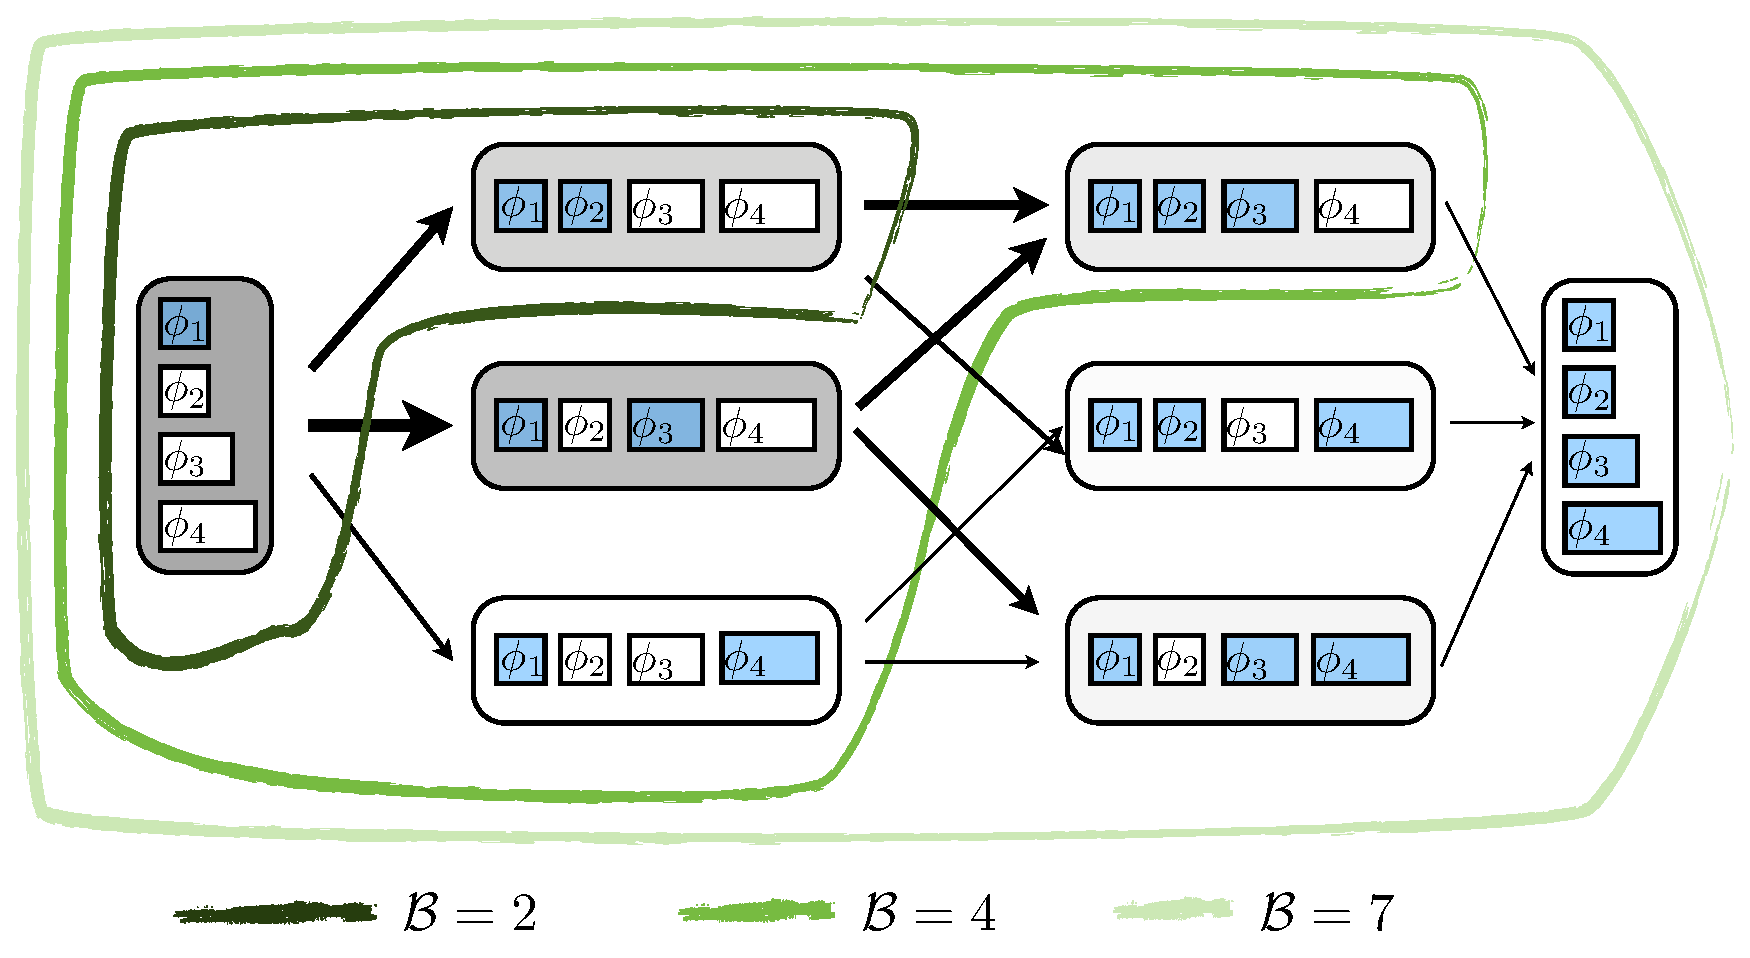
\includegraphics[width=1\linewidth]{../../figures/mdp_masks.pdf}
\caption{
The action space $\mathcal{A}$ of the MDP is the the set of features $\mathcal{H}$, represented by the $\phi$ boxes.
The primary discretization of the state space can be visualized by the possible feature subsets (larger boxes); selected features are colored in the diagram.
The feature selection policy $\pi$ induces a distribution over feature subsets, for a dataset, which is represented by the shading of the larger boxes.
Not all states are reachable for a given budget $\mathcal{B}$.
In the figure, we show three ``budget cuts'' of the state space.
\label{fig:state_space}
}
\end{figure}

%!TEX root=../paper/paper.tex
\section{Evaluation}\label{sec:ccnn_evaluation}

\PM{Dataset}
We evaluate on the standard object detection benchmark: the PASCAL VOC \cite{pascal-voc-2010}.
In all cases, the CNN region classifiers are trained on the PASCAL VOC 2007 trainval set.
The parameters of our methods are set by training or cross-validation on the VOC 2007 val set.
We evaluate on the VOC 2007 test set.
The result plots and details are shown in \autoref{fig:voc2007_results} and \autoref{tab:ccnn_results}.

\PM{Implementation}
The scoring function for the quick-to-compute features is trained by a logistic regression classifier onto the max PASCAL overlap with any ground truth window on the validation dataset.
The classifier is optimized by stochastic gradient descent, and its regularization parameter is cross-validated.
The R-CNN software was used as available in June 2014.
\footnote{\url{https://github.com/rbgirshick/rcnn}}
That software relies on Selective Search \cite{Uijlings-IJCV-2013} region proposals.
Different images are proposed different numbers of regions.
\autoref{fig:roi_hist} shows the distribution of number of regions on the validation set, with the parameters of the R-CNN.
An additional parameter is the size of each batch of regions that goes through the CNN.
We set batch size to 100 regions, and observe that it takes on average 500 ms to process them with the CNN.
In all experiments, we use Ubuntu 12.04, Intel i5 3.2GHz CPU, and NVIDIA Tesla K40 GPU.

%!TEX root=../paper/paper.tex
\begin{figure}[ht]
\begin{subfigure}[b]{\linewidth}
    \centering
    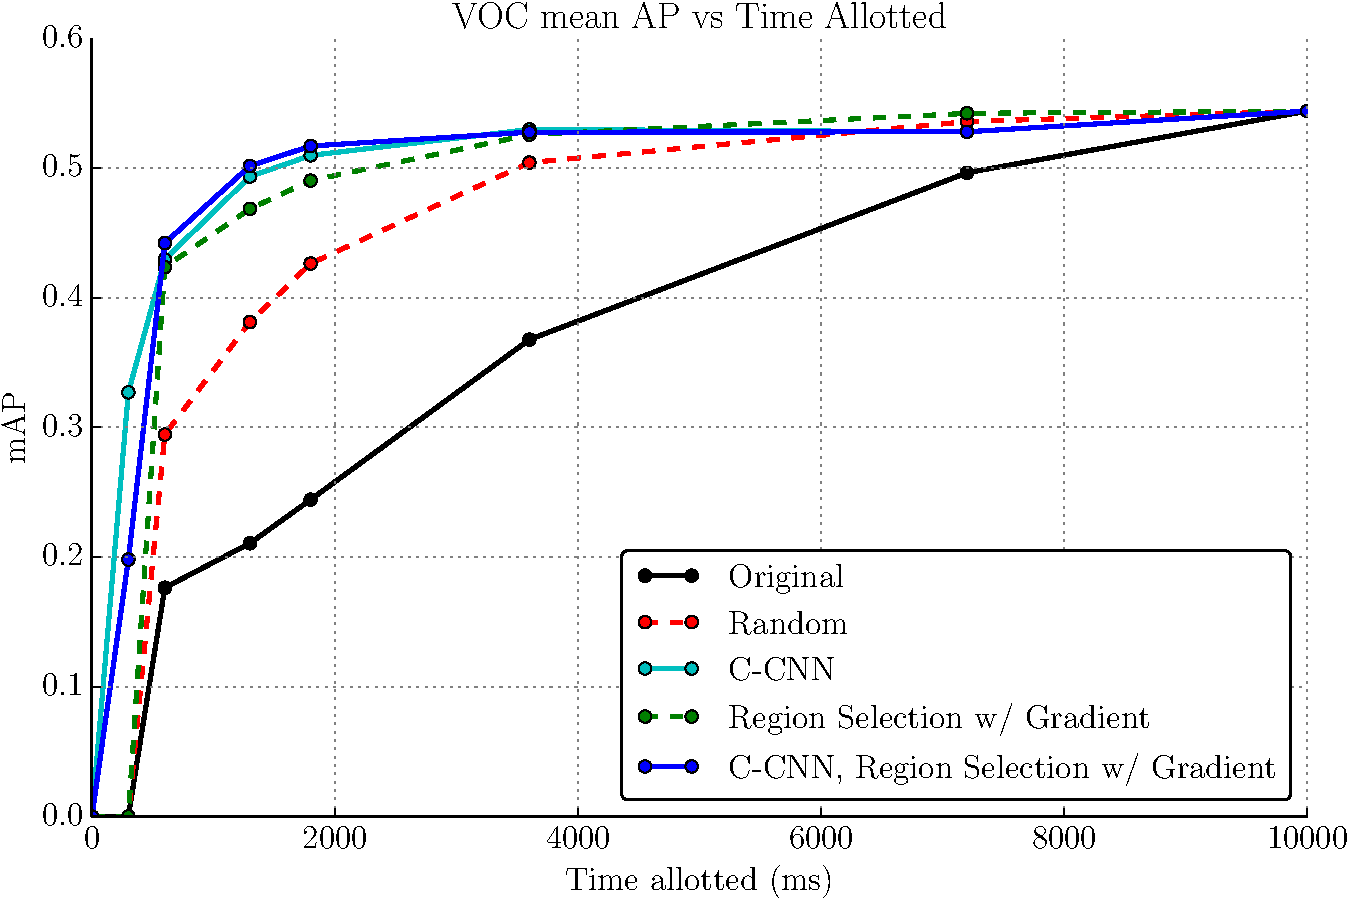
\includegraphics[width=.75\linewidth]{../ccnn/figures/_apvst_final.pdf}
    \caption{
Plotting Mean AP vs. Time Allotted allows comparison performance at a given time budget.
For example, at 1300 ms, random region selection gets about 0.42 mAP, while our best method (C-CNN with gradient-based region selection) obtains 0.50 mAP.
}\label{fig:apvst}
\end{subfigure}
\begin{subfigure}[b]{\linewidth}
    \centering
    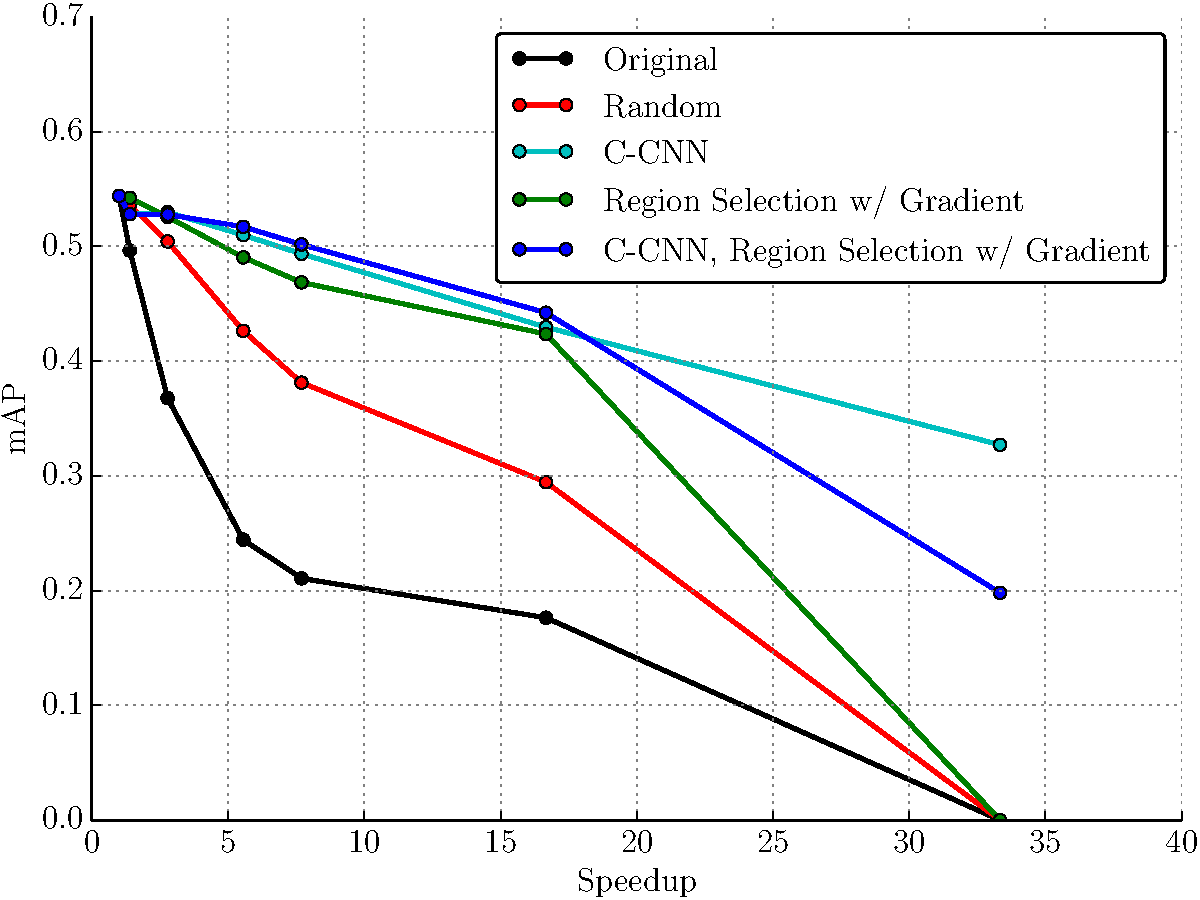
\includegraphics[width=.75\linewidth]{../ccnn/figures/_speedup_final_abs.pdf}
    \caption{
Plotting mean AP vs. speed-up factor allows comparison of speed-ups at a given mAP point.
For example, we can see that we should obtain mAP of 0.40 at around 20x speedup with our method.
}\label{fig:speedup}
\end{subfigure}
\caption{
Results of the Cascade CNN and other Anytime methods on the PASCAL VOC 2007 dataset.
}\label{fig:voc2007_results}
\end{figure}


\begin{table}[ht]
\centering
\caption{
Full table of AP vs. Time results on PASCAL VOC 2007.
Best performance for each time point is in bold.
}\label{tab:results}
\small{
\begin{tabular}{lrrrrrrrr}
\toprule
Time allotted (ms)                  & 0 & 300            & 600            & 1300           & 1800           & 3600           & 7200           & 10000 \\
\midrule
Original                            & 0 & 0.000          & 0.176          & 0.211          & 0.244          & 0.368          & 0.496          & 0.544 \\
Random                              & 0 & 0.000          & 0.295          & 0.381          & 0.426          & 0.504          & 0.536          & 0.544 \\
C-CNN                               & 0 & \textbf{0.327} & 0.430          & 0.493          & 0.510          & 0.528          & 0.528          & - \\
Region Selection w/ Gradient        & 0 & 0.000          & 0.424          & 0.469          & 0.490          & 0.526          & \textbf{0.542} & 0.544 \\
C-CNN, Region Selection w/ Gradient & 0 & 0.198          & \textbf{0.442} & \textbf{0.502} & \textbf{0.517} & \textbf{0.528} & 0.528          & - \\
\bottomrule
\end{tabular}
}
\end{table}


The experimental settings are
\begin{description}
  \item[Original] \hfill \\
  The original order of the Selective Search regions of interest.
  This order is influenced by the hierarchical segmentation of their method, and so has sequences of highly overlapping regions.

  \item[Random] \hfill \\
  A completely blind permutation of the original order.

  \item[Region Selection] \hfill \\
  The region statistics feature is always used.
  Additionally, we consider the Pixel Gradient feature, with \emph{setup time} of the gradient forward-back propagation of 20 ms.

  \item[Cascaded CNN] \hfill \\
  The Cascaded CNN model, as described in \autoref{sec:ccnn}.
  The first experiment (C-CNN) takes batches of regions in a random order.
  The next two experiments also make use of the Region Selection methodology with the quick-to-compute feature.
\end{description}

\PM{Analysis}
Since the time to process a full batch with a non-cascaded CNN is 500 ms, there are no results for non-cascaded baselines at 300 ms.
At this time, the Cascaded CNN without any region ordering is best.
A reason for why C-CNN with Region Selection is not as good at this point is that the region selection presents better region candidates, with fewer rejection opportunities, and thus has less coverage of the image.
At 600 ms, C-CNN method have had more than one batch go through, and the Region Selection is giving it a lead over the simple C-CNN.
Both method are better than the baseline non-cascaded methods for this entire duration.

%!TEX root=paper/paper.tex
\chapter{Conclusion}\label{sec:conclusion}

\PM{Contribution}
We note a significant problem that has received little research attention: Anytime visual recognition.
The problem is motivated by the properties of human visual perception and by the need to effectively schedule computationally expensive state-of-the-art computer vision methods for different computational budgets.
We approach the problem from the perspective of reinforcement learning, and successfully learn fully general policies for selecting detector and classifier actions.
To evaluate our approaches, we introduce a new metric of Anytime performance, based on the area of performance vs. cost curve.
In all experiments, we show that having a dynamic state (allowing closed-loop policies) and planning ahead increases performance.

\PM{Detection}
We present a method for learning ``closed-loop'' policies for multi-class object detection, given existing object detectors and classifiers and a metric to optimize.
The method learns the optimal policy using reinforcement learning, by observing execution traces in training.
As always with reinforcement learning problems, defining the reward function requires some manual work.
Here, we derive it for the novel detection AP vs. Time evaluation that we suggest is useful for evaluating efficiency in recognition.
If detection on an image is cut off after only half the detectors have been run, our method does $66\%$ better than a random ordering, and $14\%$ better than an intelligent baseline.
In particular, our method learns to take action with no intermediate reward in order to improve the overall performance of the system.

\PM{Classification}
For the classification task, we additionally need to train classifiers for partially-observed sets of features.
We investigate methods such as different forms of imputation and classifier clustering for this task, and adjust the reward function and the featurization of the state.
We show improved Anytime performance on one synthetic classification task and two real visual recognition tasks using our method.
On a hierarchically-structured dataset, we additionally show that accuracy of predictions can be held constant for all budgets, while the specificty of predictions increases.

\PM{C-CNN}
We first consider approaches which can effectively reorder the sequence of regions to maximize the chance that correct detections will be found early, based on inference from relatively lightweight features.
We show that basic strategies, such as simply randomly reordering the boxes such that they do not have a degenerate spatial layout, provides a surprising boost, and that very simple features such as region and gradient statistics can effectively prioritize regions.
The main contribution, however, is the Cascaded CNN model, which adds a novel Reject layer to the AlexNet architecture and obtains an almost 10x speedup of the R-CNN detection method with only a 10\% degradation of state-of-the-art performance on PASCAL VOC detection.

\section{Future work}

\PM{Decisions}
Although computation devoted to scheduling actions is less significant than the computation due to running the actions in all of our work, our framework does not explicitly consider this decision-making cost.
A welcome extension would explicitly model this, perhaps drawing on eixsting theoretical work on meta-reasoning \parencite{Hay2012}.
This principle can also be applied to neural networks; we currently learn rejection thresholds in a process separate from the CNN training.
Future work should learn these thresholds jointly with the convolutional filters and the rest of the network layers.

\PM{Classification}
Nearest-neighbor method work really well for settings with partially observed sets of features, but were too slow in our evaluation.
Locality-sensitive hashign methods may provide an effective solution.
In particular, the method of \cite{Gao-NIPS-2011} could be valuably extended with hashing to maintain its model-free advantages at an acceptable speed.

\PM{Perception}
Beyond the aspects of practical deployment of vision systems that our work is motivated by, we are curious to further investigate our model as a tool to study human cognition and the time course of visual perception.
Only a few attempts have been made to explain this: for example, via sequential decision processes in \textcite{Hegde-Neuro-2008}.
While we have not made any claims about the biological mechanism of perception, our work in reinforcement learning-based feature selection as well as convolutional neural networks has explanatory potential if more tightly integrated in future work.


{\small
\section*{Acknowledgements}
This research was supported by the National Defense Science and Engineering Graduate Fellowship; DARPA Mind's Eye and MSEE programs; NSF awards IIS-0905647, IIS-1134072, and IIS-1212798; by Toyota; and by the Intel Visual Computing Institute.

\bibliographystyle{ieee}
\bibliography{../sergeyk_library}
}
